\documentclass[../../main]{subfiles}
\graphicspath{{\subfix{../../Images/}}}

\begin{document}

W tej części pracy zostanie szczególnie omówiona i przeanalizowana jedna z części nadzorcy — planista, zostaną przedstawione i omówione algorytmy zarządzania zasobami jednostki obliczeniowej realizowane przez planistę. Pojęcie zasobu jednostki obliczeniowej jest wyjaśnione w \hyperref[sec:zalacznik-4]{załączniku nr 4}.

\subsection{Rodzaje algorytmów}

\subsubsection{Techniki wielordzeniowe}

Najpierw należy zauważyć, że jeden system może zawierać więcej niż jedną jednostkę obliczeniową. Jednostki te mogą być zorganizowane w sposób umożliwiający równoczesne wykonywanie instrukcji procesów dostępnych dla wszystkich jednostek (tzw. wielordzeniowość; ang. multicore). W takich przypadkach są stosowane techniki \gls{amp} lub \gls{smp}.

Na \cref{fig:amp-smp} przedstawiono różnię pomiędzy \gls{amp} a \gls{smp}. W przypadku \gls{amp} każdej jednostce obliczeniowej przypisywany jest oddzielny proces, natomiast w przypadku \gls{smp} każdy proces jest dzielony na wątki, a każdemu wątkowi przypisywane są zasoby poszczególnych jednostek obliczeniowych.

W niniejszej pracy techniki \gls{smp} nie będą omawiane, ponieważ ich zastosowanie wymaga, aby zarówno oprogramowanie systemowe, jak i program uruchamiany na jego podstawie, były napisane z myślą o użycie wątków (np. POSIX PThreads, znany także jako IEEE 1003.1c-1995). Z jednej strony wprowadza ona znaczne skomplikowanie, a z drugiej strony nie wprowadza znacznych zmian w algorytmy zarządzania zasobami jednostki obliczeniowej. Zmiana polega jedynie na tym, że zamiast przypisywania zasobów procesom, planista przydziela je wątkom, które z punktu widzenia planisty nie różnią się od procesów. Zarówno wątki, jak i procesy posiadają listę instrukcji do wykonania, stos oraz metadane interpretowane przez planistę.

\begin{figure}[ht]
    \centering
    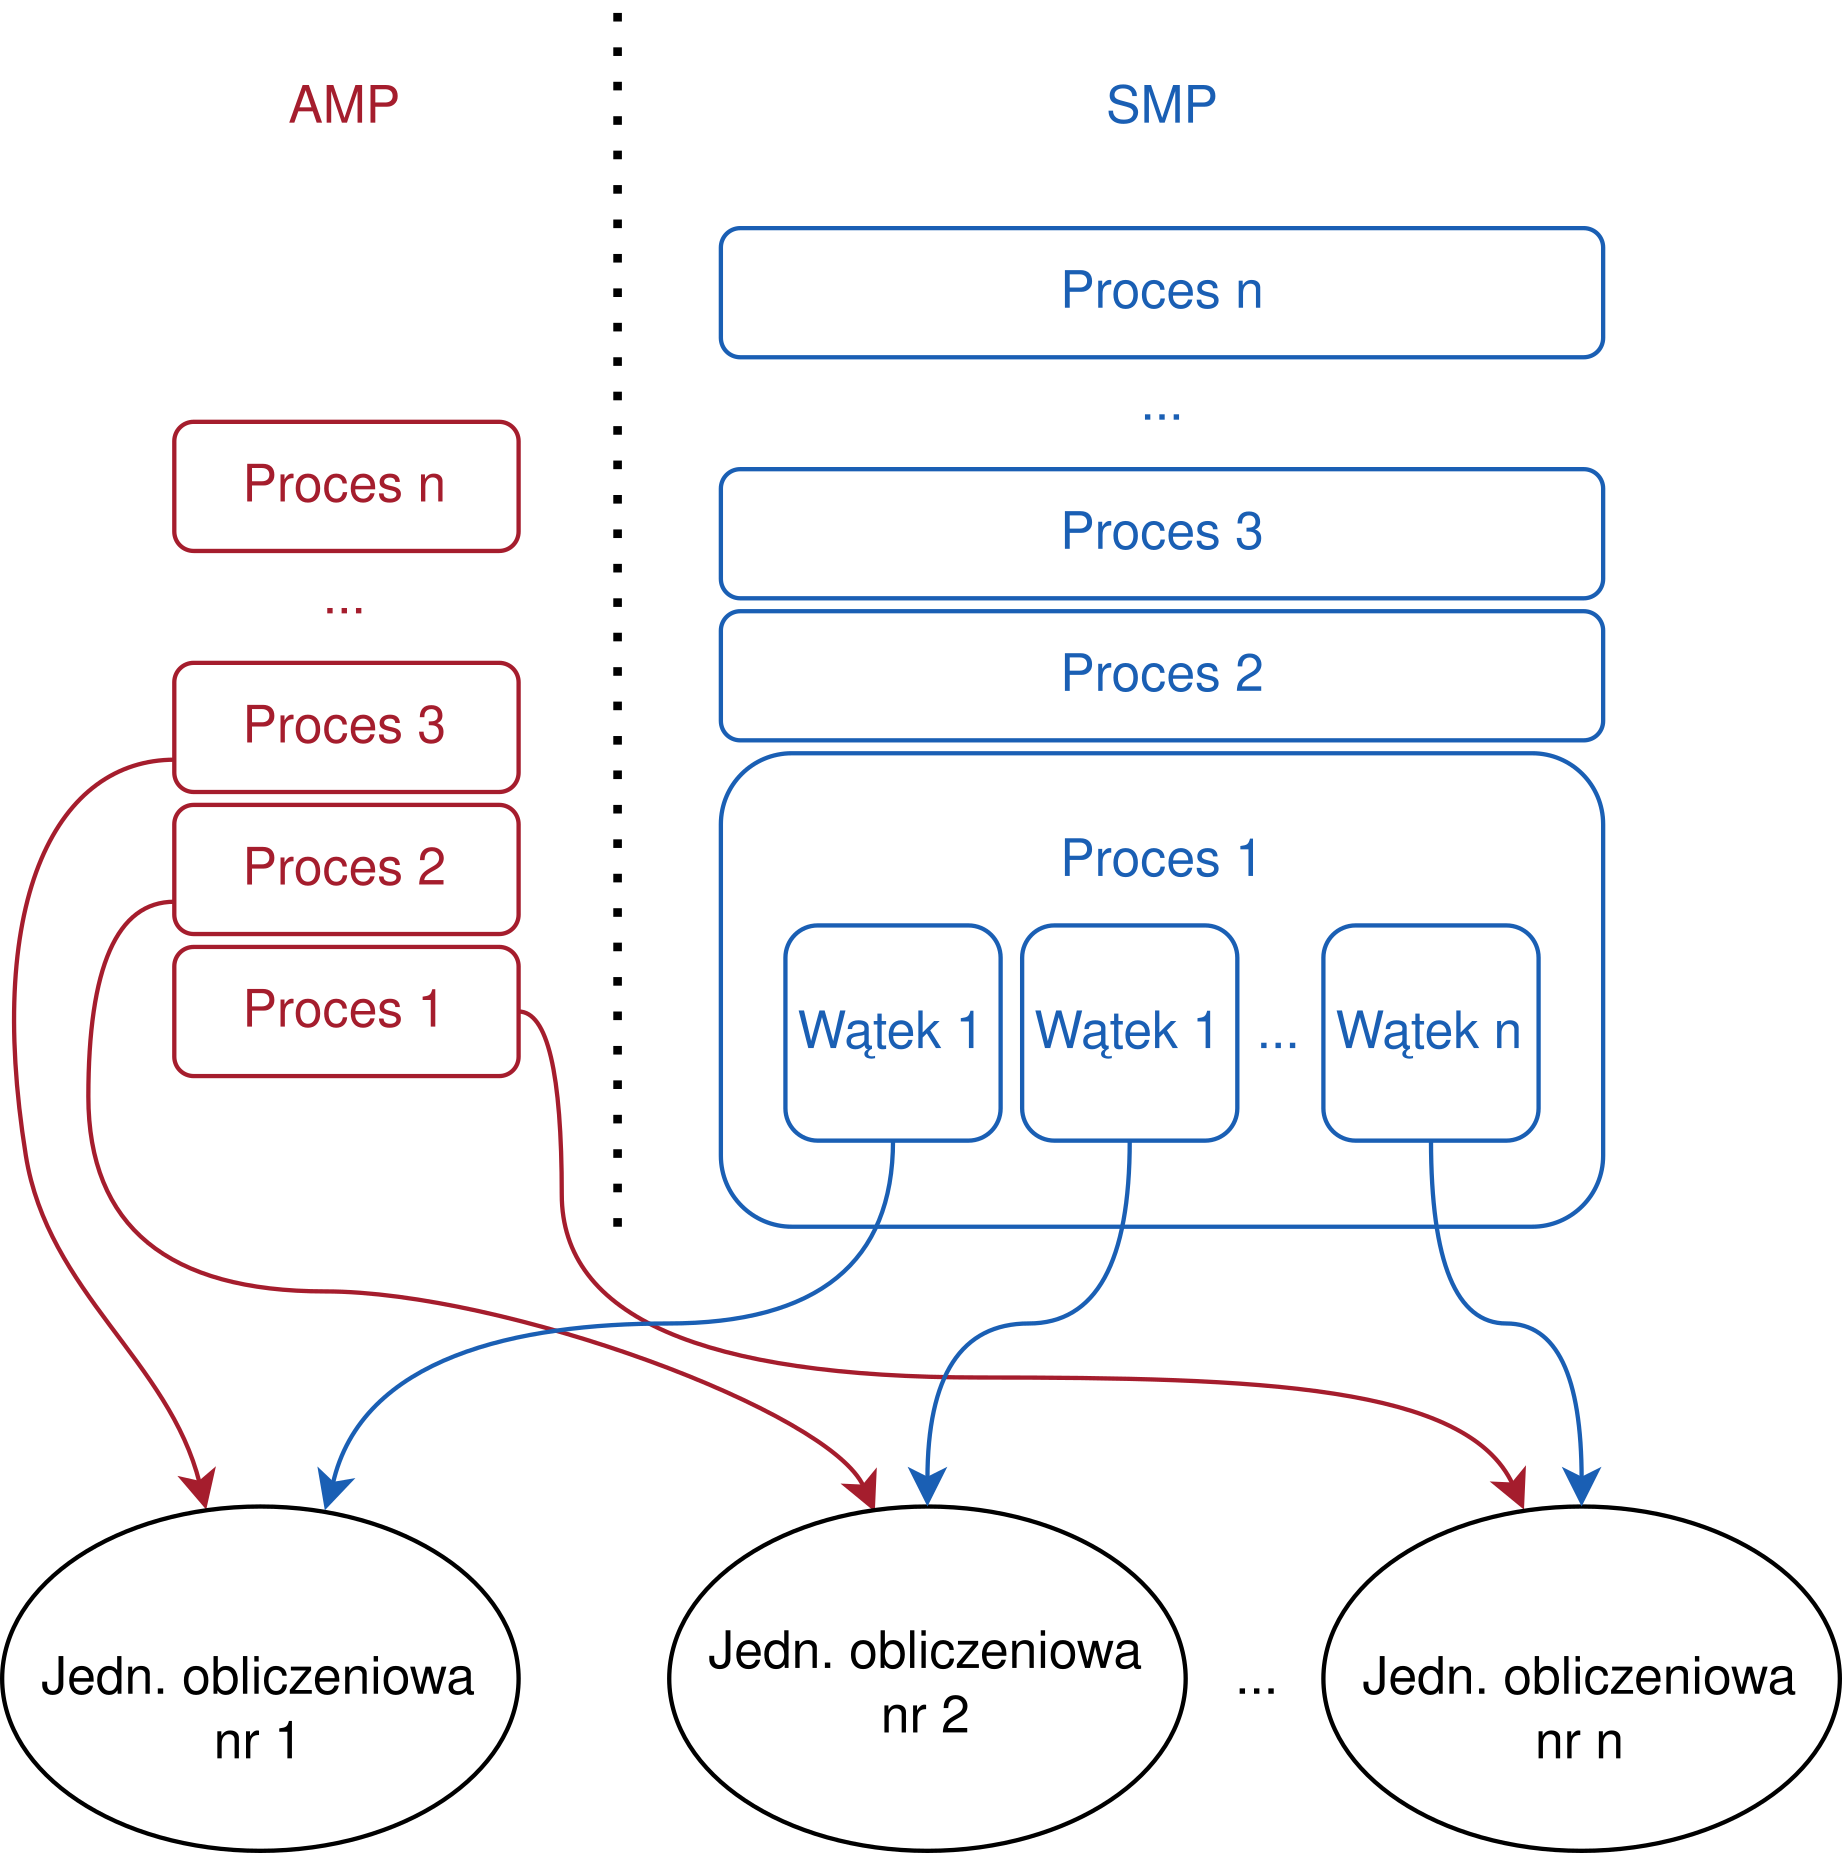
\includegraphics[width=0.80\textwidth]{Images/amp-smp.png}
    \caption{Różnica pomiędzy technikami AMP i SMP}
    \label{fig:amp-smp}
\end{figure}

Więc, w ramach niniejszej pracy, w przypadku obecności wielu jednostek obliczeniowych,analizowane będą wyłącznie techniki \gls{amp}.

\subsubsection{Techniki AMP}

\gls{amp} oznacza, że każdej jednostce obliczeniowej przypisany jest jeden proces \cref{fig:amp-smp}. Powstaje wtedy pytanie: kiedy i w jaki sposób każdemu procesowi przydzielana jest jednostka obliczeniowa? 

Istnieją dwie zupełnie różne techniki rozwiązujące ten problem: partycjonowanie statyczne (ang. static partitioning scheduling; \cref{fig:static-semistatic}) oraz zarządzanie globalne (global scheduling \cref{fig:dynamic-scheduling}). Oprócz nich istnieje także trzecia technika, wymyślona w celu zaadresowania problemów poprzednich dwóch technik — partycjonowanie dynamiczne (ang. dynamic partitioning, znana również jako ang. semi-static partitioning; \cref{fig:static-semistatic}). \cite{saranya-hansdah}

Partycjonowanie statyczne opiera się na podziale jednostek obliczeniowych pomiędzy wszystkie procesy jeszcze przed uruchomieniem nadzorcy. Typowo, tworzone są kolejki przypisane do każdej jednostki obliczeniowej (\cref{fig:static-semistatic}). Decyzja o tym, jaki proces otrzyma zasoby jednostki obliczeniowej z danej kolejki, należy do planisty, który zarządza wykonaniem procesów w każdej z kolejek. Głównym problemem tego podejścia jest sytuacja, w której wszystkie procesy w pewnych kolejkach znajdują się w stanie nieaktywnym — wówczas jednostki obliczeniowe przypisane do tych kolejek pozostają niewykorzystane, co prowadzi do marnowania zasobów.

\begin{figure}[ht]
    \centering
    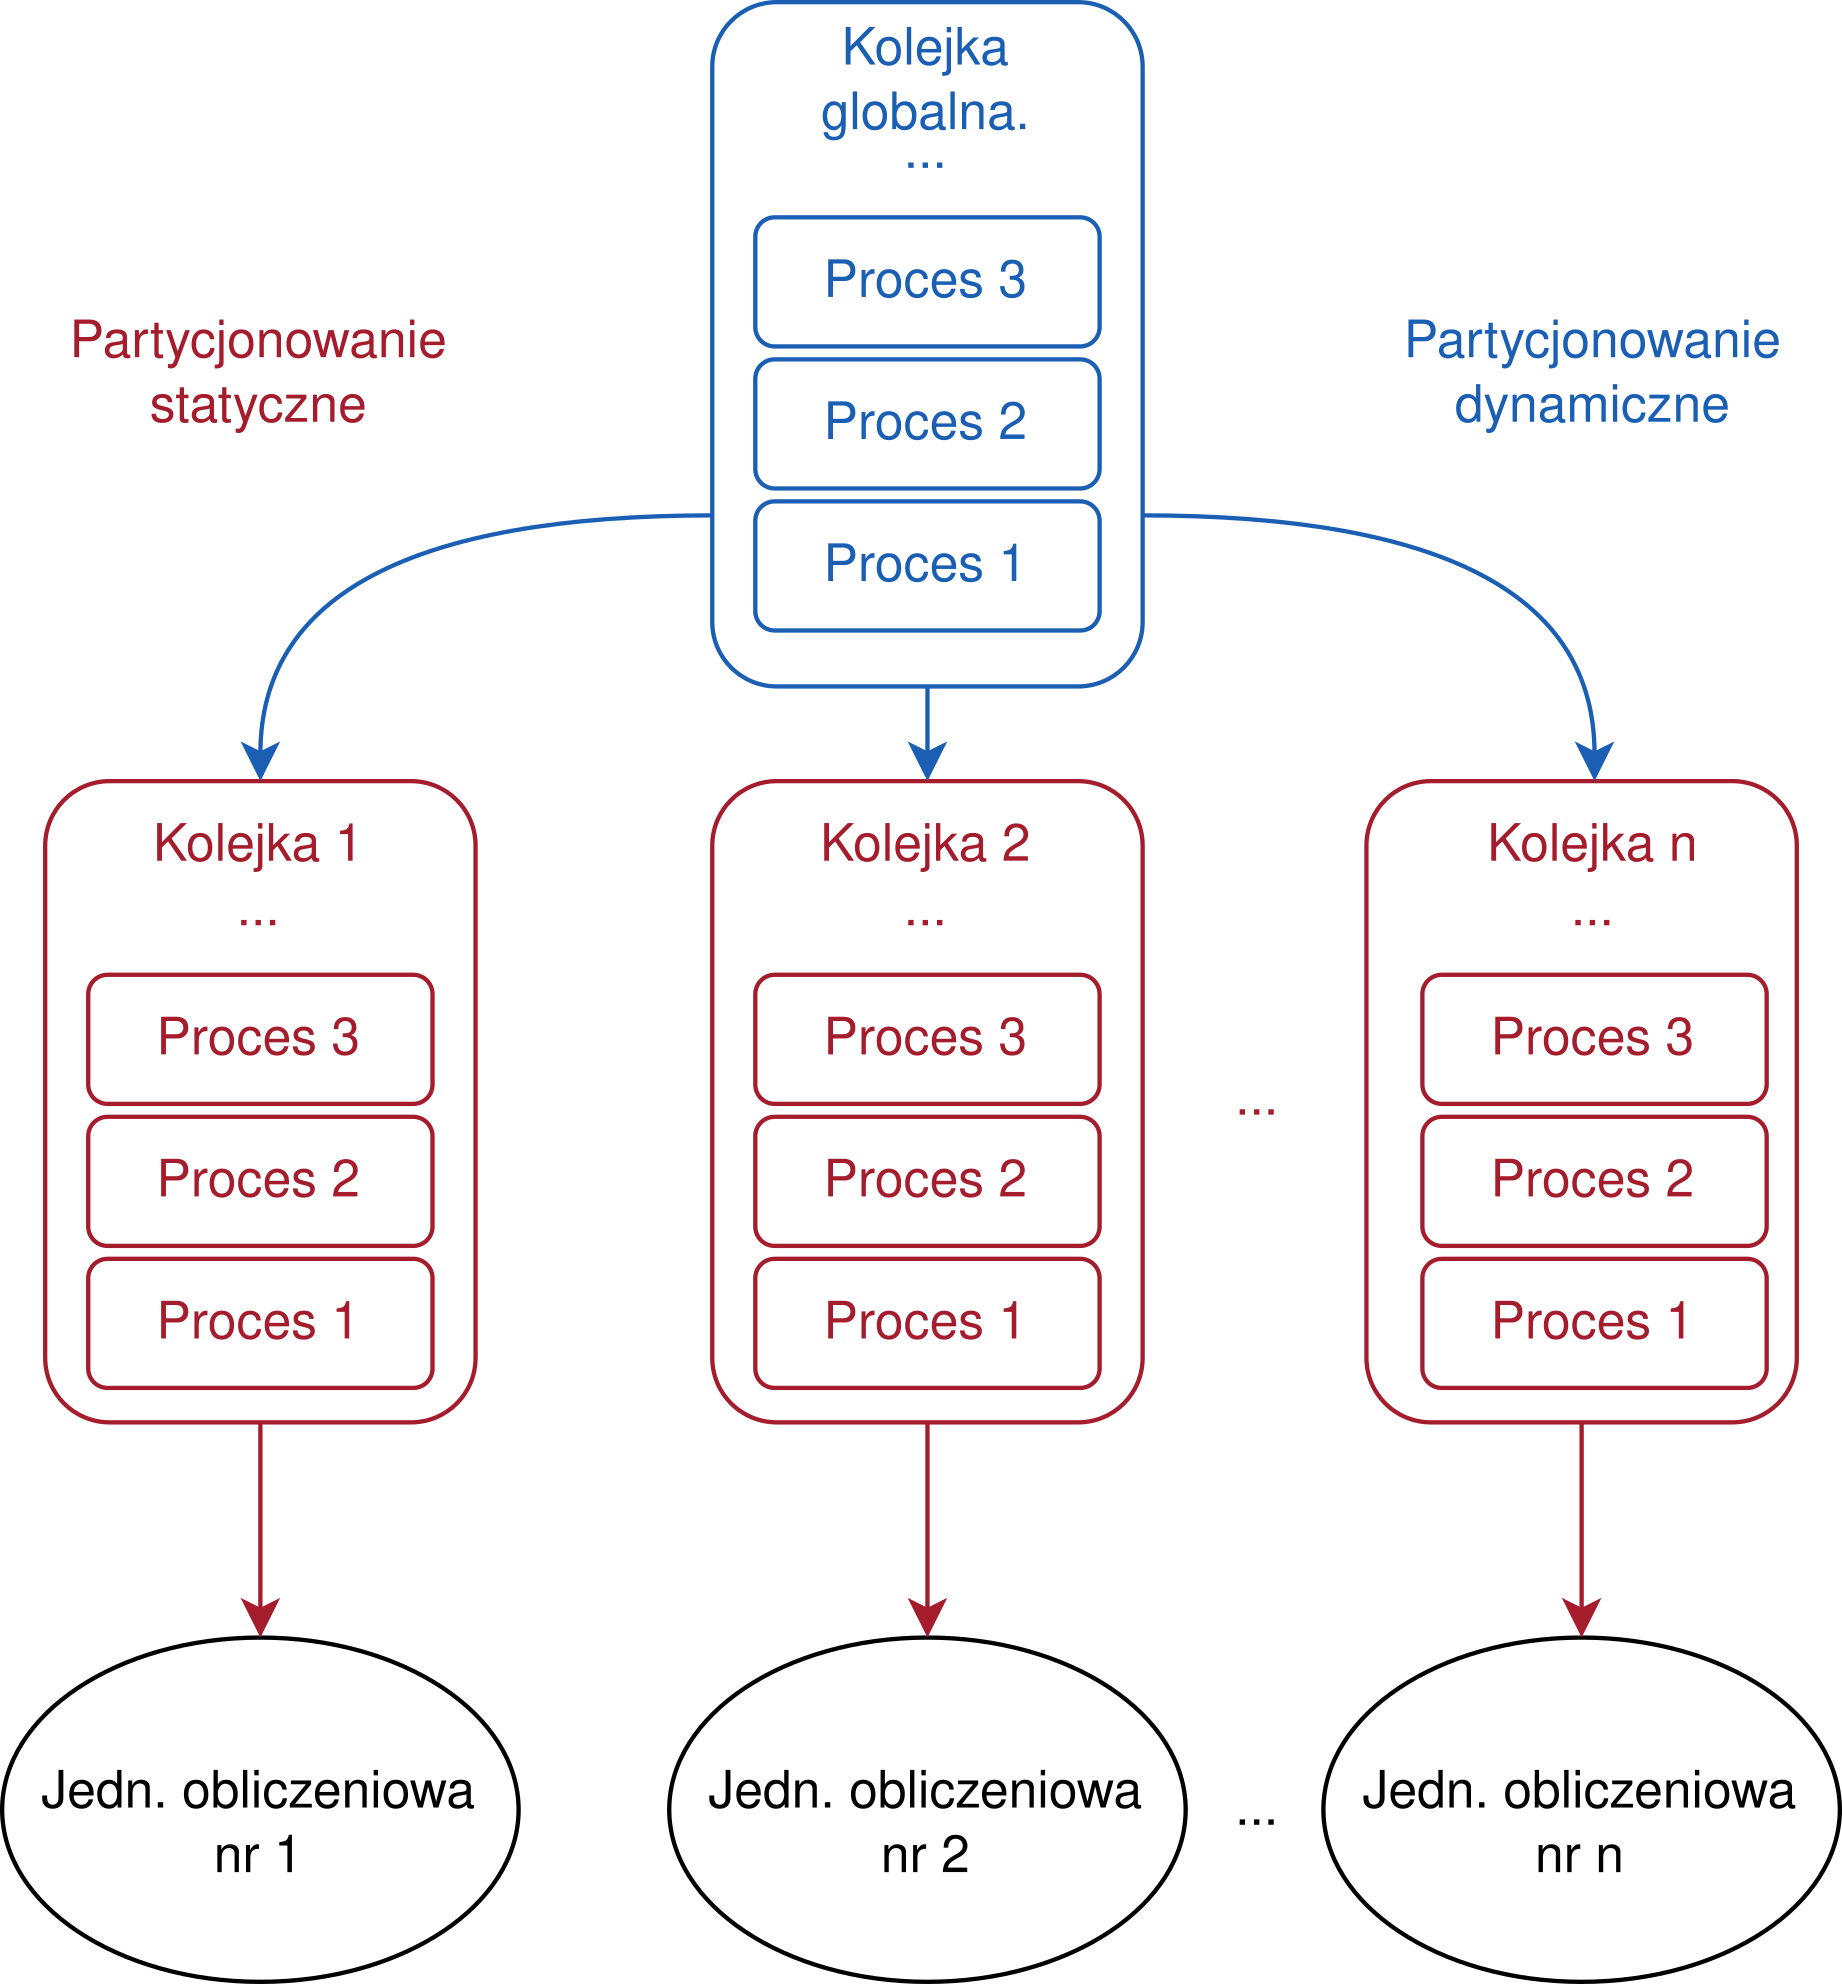
\includegraphics[width=0.80\textwidth]{Images/static-semistatic.png}
    \caption{Techniki AMP: partycjonowanie statyczne i partycjonowanie dynamiczne}
    \label{fig:static-semistatic}
\end{figure}

Zarządzanie globalne opiera się na jednym planiście, który przydziela zasoby wszystkich jednostek obliczeniowych procesom znajdującym się w jednej wspólnej kolejce (\cref{fig:dynamic-scheduling}). Głównym problemem tego podejścia jest migracja zadań pomiędzy jednostkami obliczeniowymi, która wymaga realizacji skomplikowanej logiki. Powoduję to nadużycie zasobów obliczeniowych przez planistę i dystrybutora.

Partycjonowanie dynamiczne jest połączeniem dwóch wcześniej opisanych technik. Używane są kolejki dla każdej z dostępnych jednostek obliczeniowych, zgodnie z tym, jak to jest robione w partycjonowaniu statycznym, oraz kolejka globalna, podobna do tej stosowanej w zarządzaniu dynamicznym. Pomysł polega na podziale procesów na dwie grupy: procesy, które są statycznie przywiązane do określonej jednostki obliczeniowej, oraz procesy, które "wędrują" pomiędzy jednostkami obliczeniowymi. Celem tej techniki jest minimalizacja skutków problemów opisanych w poprzednich technikach:

\begin{itemize}
    \item Jeśli procesy w statycznie zdefiniowanej kolejce będą nieaktywne, proces z kolejki globalnej zostanie przydzielony do swobodnej jednostki obliczeniowej.
    \item Ponieważ w kolejce globalnej znajduje się tylko część procesów, częstość migracji procesów będzie zmniejszona, co oznacza, że mniej czasu będzie marnowane na działanie planisty i dyspozytora.
\end{itemize}

\begin{figure}[ht]
    \centering
    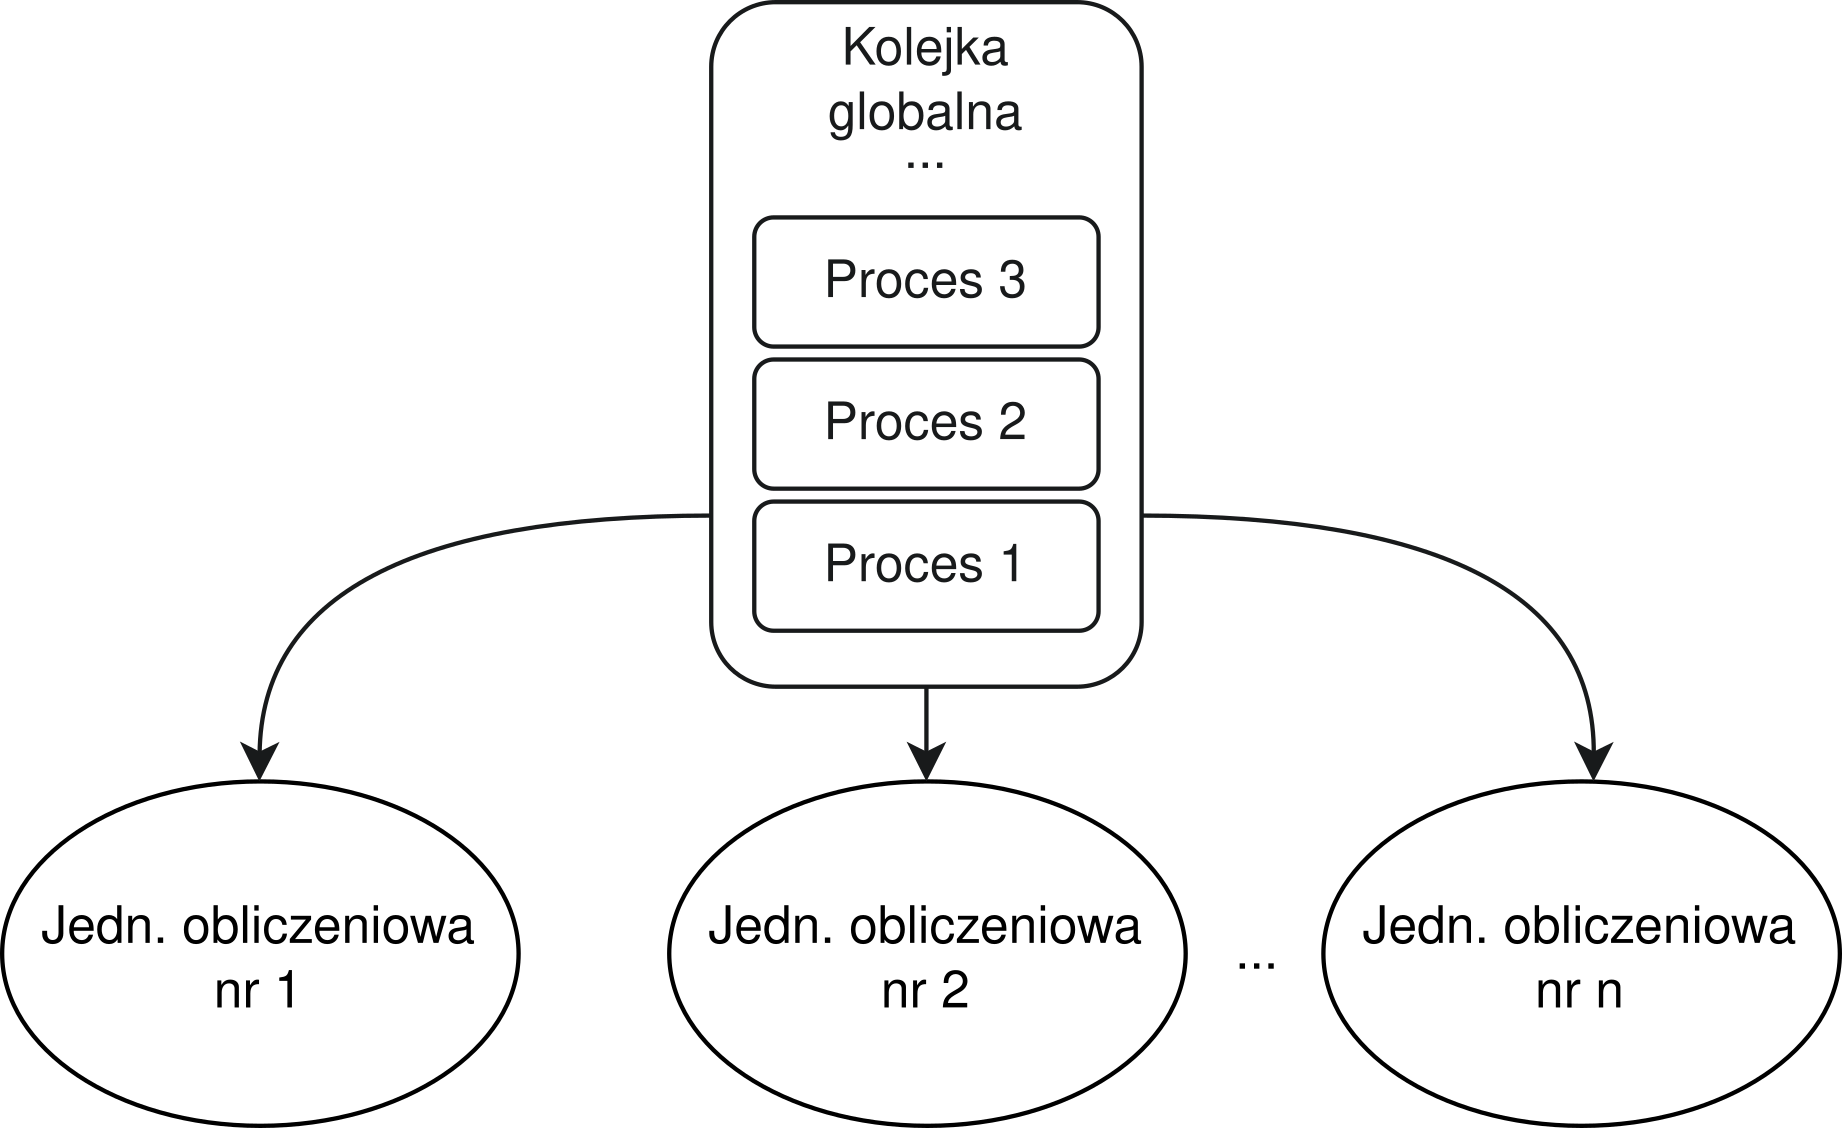
\includegraphics[width=0.80\textwidth]{Images/dynamic-scheduling.png}
    \caption{Technika AMP: zarządzanie globalne}
    \label{fig:dynamic-scheduling}
\end{figure}

Te techniki nie definiują, dlaczego i w jaki sposób każdy proces otrzymuję zasoby jednostki obliczeniowej, lecz określają sposoby rozprowadzenia obciążenia w systemie z wieloma jednostkami obliczeniowymi. Algorytmy przypisywania zasobów poszczególnych jednostek obliczeniowych do przypisanych do tych jednostek procesów są ukryte w planistach przypisanych do każdej kolejki i nazywane są technikami jednordzeniowymi. Będzie to omówione w następnej części pracy. % TODO: defniniują, dlaczego

\subsubsection{Techniki jednordzeniowe}

W przypadku, gdy w systemie jest obecna tylko jedna jednostka obliczeniowa lub gdy zachodzi potrzeba zaimplementowania planisty dla poszczególnych kolejek w technikach AMP, jest mowa o technikach jednordzeniowych. Techniki te można podzielić na grupy, które posiadają niektóre z właściwości pokazanych na \cref{fig:uniprocessor-technics}.

Wywłaszczenie to właściwość, która pozwala nadzorcy na interwencję w wykonywanie procesu i jego podmianę na inny proces, kiedy poprzedni jeszcze nie osiągnął swojego celu. Taka właściwość umożliwia planistowi podejmowanie decyzji o tym, który proces będzie wykonywany następnie, periodycznie, a nie tylko po zakończeniu wykonywania każdego z procesów.

Priorytet pozwala na nierównomierne traktowanie procesów przy przypisywaniu im zasobów jednostki obliczeniowej, co wprowadza dodatkowe możliwości optymalizacji algorytmów w zależności od określonych celów. Priorytety mogą być statyczne, zdefiniowane przed uruchomieniem nadzorcy, lub dynamiczne, przeliczane w czasie wykonywania nadzorcy.

Lista przykładowych algorytmów:

\begin{itemize}
    \item FCFS — ang. First Come First Served, to algorytm bezpriorytetowy, liniowy, niewykorzystujący wywłaszczenia. Zasada działania: proces, który jako pierwszy trafia do kolejki, otrzymuje tyle czasu, ile potrzebuje na osiągnięcia swojego celu, a kolejne procesy są obsługiwane w takiej samej kolejności. Ten algorytm nie interpretuje żadnych metadanych procesu, tylko przydziela czas jednostki obliczeniowej pierwszemu procesowi w kolejce.
    \item SJF — ang. Shortest Job First, jest to algorytm z priorytetami statycznymi, niewykorzystujący wywłaszczenia. Zasada działania: podczas przełączania kontekstu wybierany jest proces, który ma najmniejszy czas potrzebny na zakończenie zadania. Algorytm zakłada, że czas wykonania procesu jest znany przed rozpoczęciem jego realizacji.
    \item SRTN — ang. Shortest Remaning Time Next, to algorytm z dynamicznymi priorytetami i wywłaszczeniem. Zasada działania: podczas przełączania kontekstu wybierany jest proces, który ma najmniejszy czas pozostały do zakończenia zadania. Ponieważ czas pozostały do wykonania procesu zmienia się za każdym razem, gdy proces otrzymuje czas jednostki obliczeniowej, priorytet jest dynamiczny. Algorytm zakłada, że podczas przełączenia kontekstu dostępna będzie informacja o czasie pozostałym do zakończenia wykonywania procesu.
    \item RR — ang. Round Robin, algorytm bezpriorytetowy wykorzystujący wywłaszczanie. Zasada działania: każdemu procesowi przypisywana jest określona część zasobów jednostki obliczeniowej (tzw. kwant czasu). Gdy proces zużyje przypisany kwant, jednostka obliczeniowa jest przekazywana do kolejnego procesu w kolejce, i tak w kółko, dopóki każdy proces nie zakończy swojego wykonywania.
    \item RM — ang. Rate-Monotonic, algorytm ze statycznymi priorytetami wykorzystujący wywłaszczanie. Zasada działania: priorytet jest obliczany przed uruchomieniem nadzorcy, najwyższy priorytet ma proces o najmniejszej częstości pojawienia w systemie (ang. rate); proces o wyższym priorytecie wywłaszcza proces o mniejszym priorytecie i używa zasobów jednostki obliczeniowej, dopóki nie osiągnie swojego celu; następnie do wykonania zostaje przewrócony proces o niższym priorytecie. Ten algorytm zakłada, że częstość pojawienia się procesu w systemie jest znana.
    \item DM — ang. Deadline-Monotonic, algorytm ze statycznymi priorytetami wykorzystujący wywłaszczanie. Zasada działania: priorytet jest obliczany przed uruchomieniem nadzorcy, najwyższy priorytet ma proces z najkrótszym najgorszym czasem osiągnięcia celu (ang. deadline); proces o wyższym priorytecie wywłaszcza proces o niższym i używa zasobów jednostki obliczeniowej, dopóki nie osiągnie swojego celu; następnie do wykonania zostaje przewrócony proces o niższym priorytecie. Ten algorytm zakłada, że najgorszy cas osiągnięcia celu przez proces w systemie jest znany.
    \item EDF — ang. Earliest Deadline First, algorytm wykorzystujący dynamiczne priorytety i wykorzystujący lub niewykorzystujący wywłaszczanie, co zależy od konfiguracji. Zasada działania: najwyższy priorytet otrzymuję proces o najbliższym najgorszym terminie osiągnięcia celu (ang. deadline).
    \item LST lub LLF — ang. Least Slack Time lub Least Laxity First, algorytm wykorzystujący dynamiczne priorytety i wykorzystujący lub niewykorzystujący wywłaszczenie, co zależy od konfiguracji. Zasada działania: najwyższy priorytet otrzymuje proces, który ma najmniejszy czas pomiędzy osiągnięciem celu a najgorszym terminem osiągnięcia celu.
    \item DARTS — ang. Dynamic Real Time Task Scheduling, algorytm wykorzystujący dynamiczne priorytety i wywłaszczenie. Jest to połączenie algorytmów EDF i LLF, w którym uwzględniany jest ostateczny termin osiągnięcia celu przez proces. Dokładniejsza zasada działania tego algorytmu będzie wyjaśniona w następnej części pracy. \cite{darts}
\end{itemize}

\begin{figure}[ht]
    \centering
    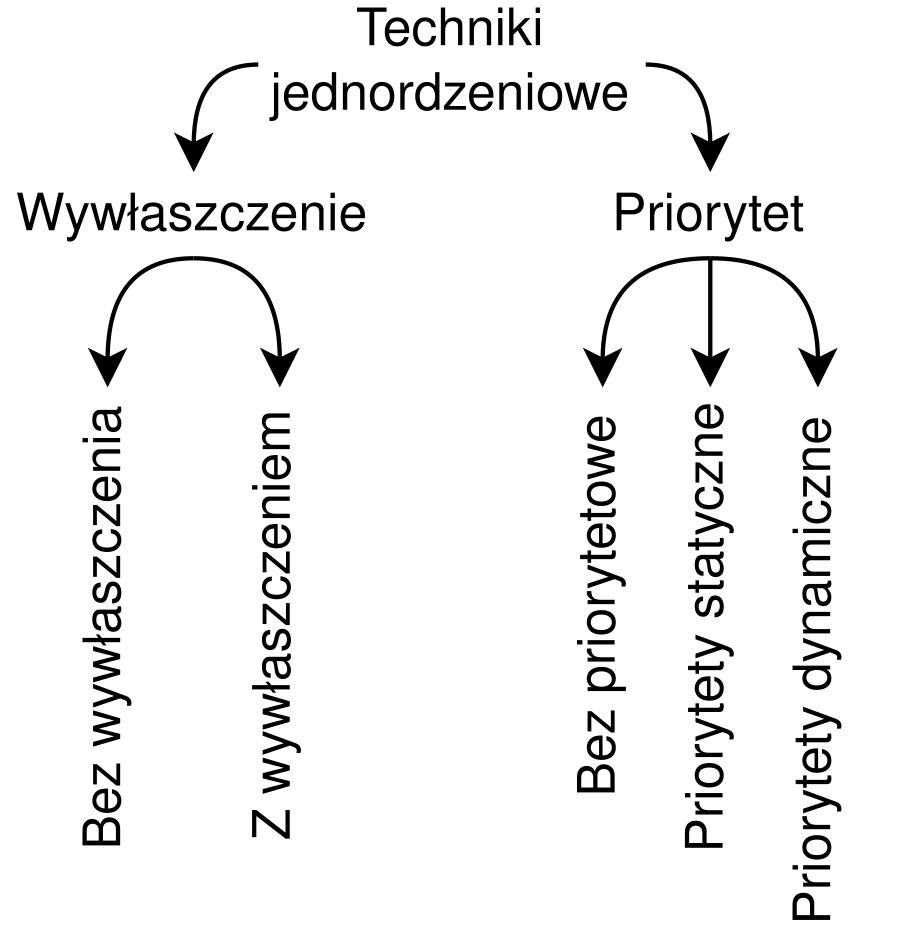
\includegraphics[width=0.50\textwidth]{Images/uniprocessor-technics.png}
    \caption{Techniki jednordzeniowe}
    \label{fig:uniprocessor-technics}
\end{figure}

Istnieje kilka sposobów przeprowadzenia analizy algorytmów zarządzania zasobami jednostki obliczeniowej w systemach operacyjnych, m.in. analiza matematyczna i symulacja. Natomiast w ramach tej pracy zdecydowano przeprowadzić analizę na podstawie realnego systemu, odpowiednio go modyfikując, co zostanie opisane w następnej części pracy.

\end{document}